\begin{figure*}[p]
\centering
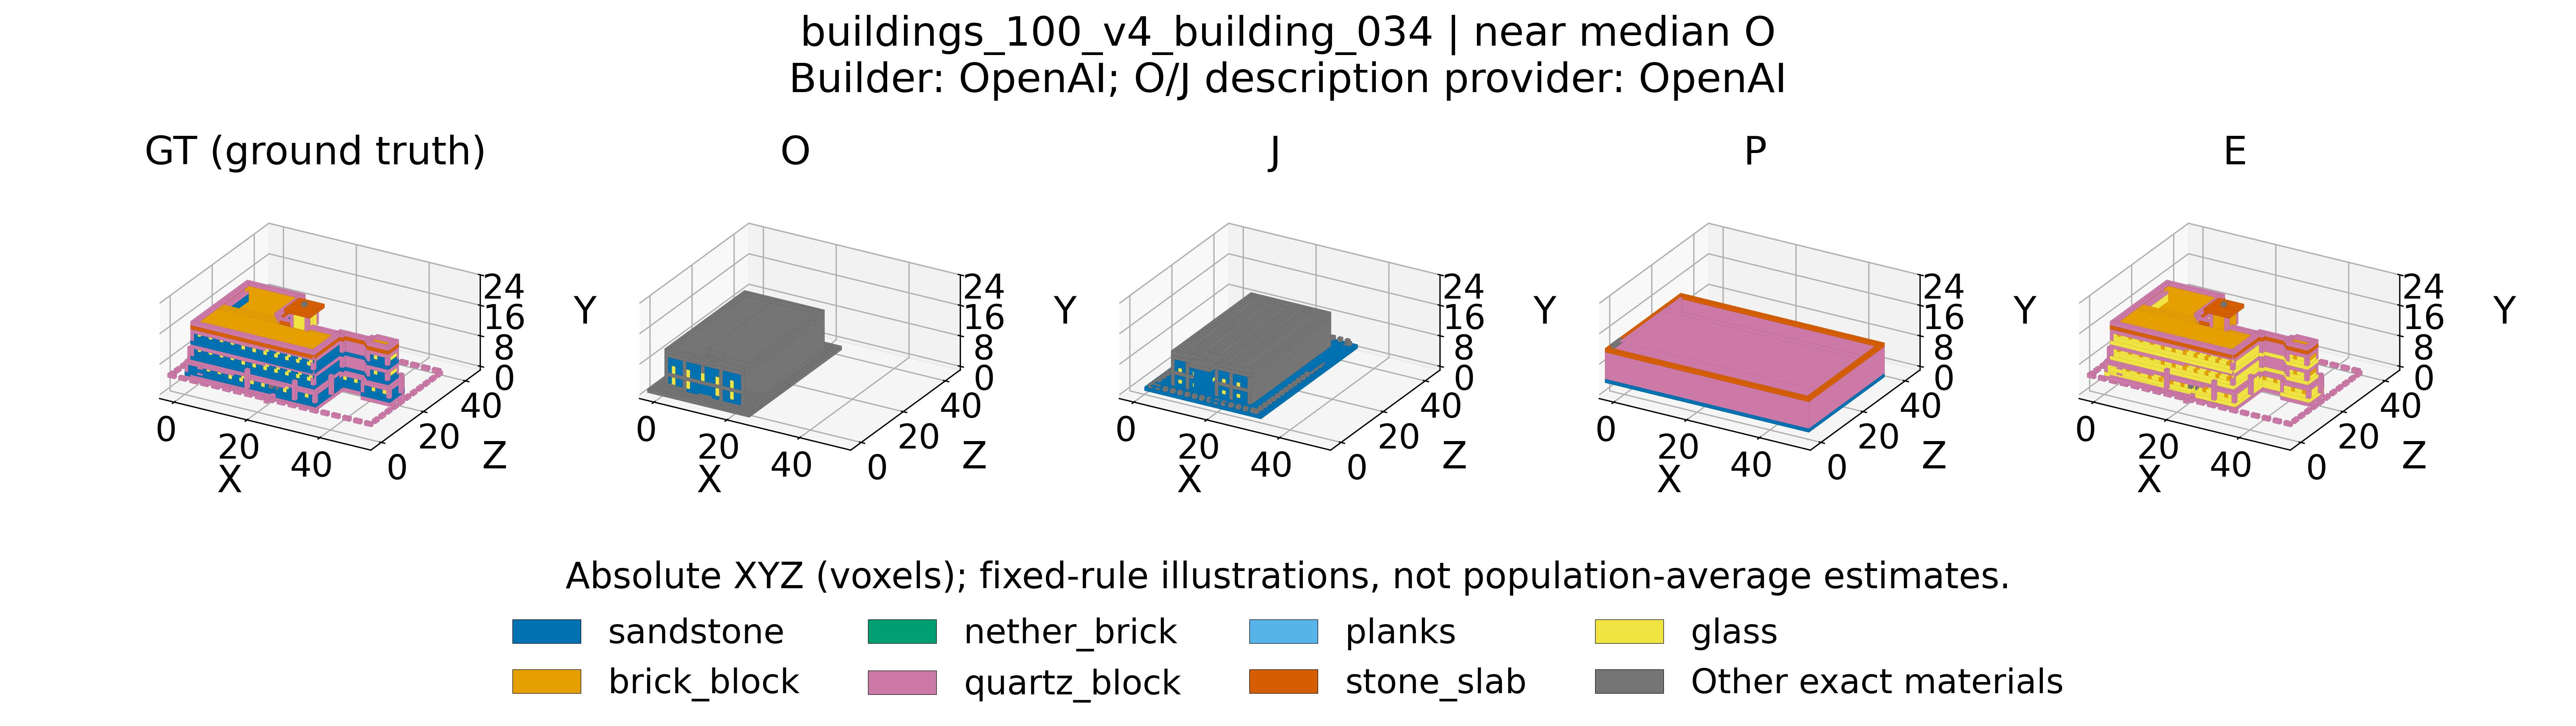
\includegraphics[width=\textwidth]{example_01.png}\\[2pt]
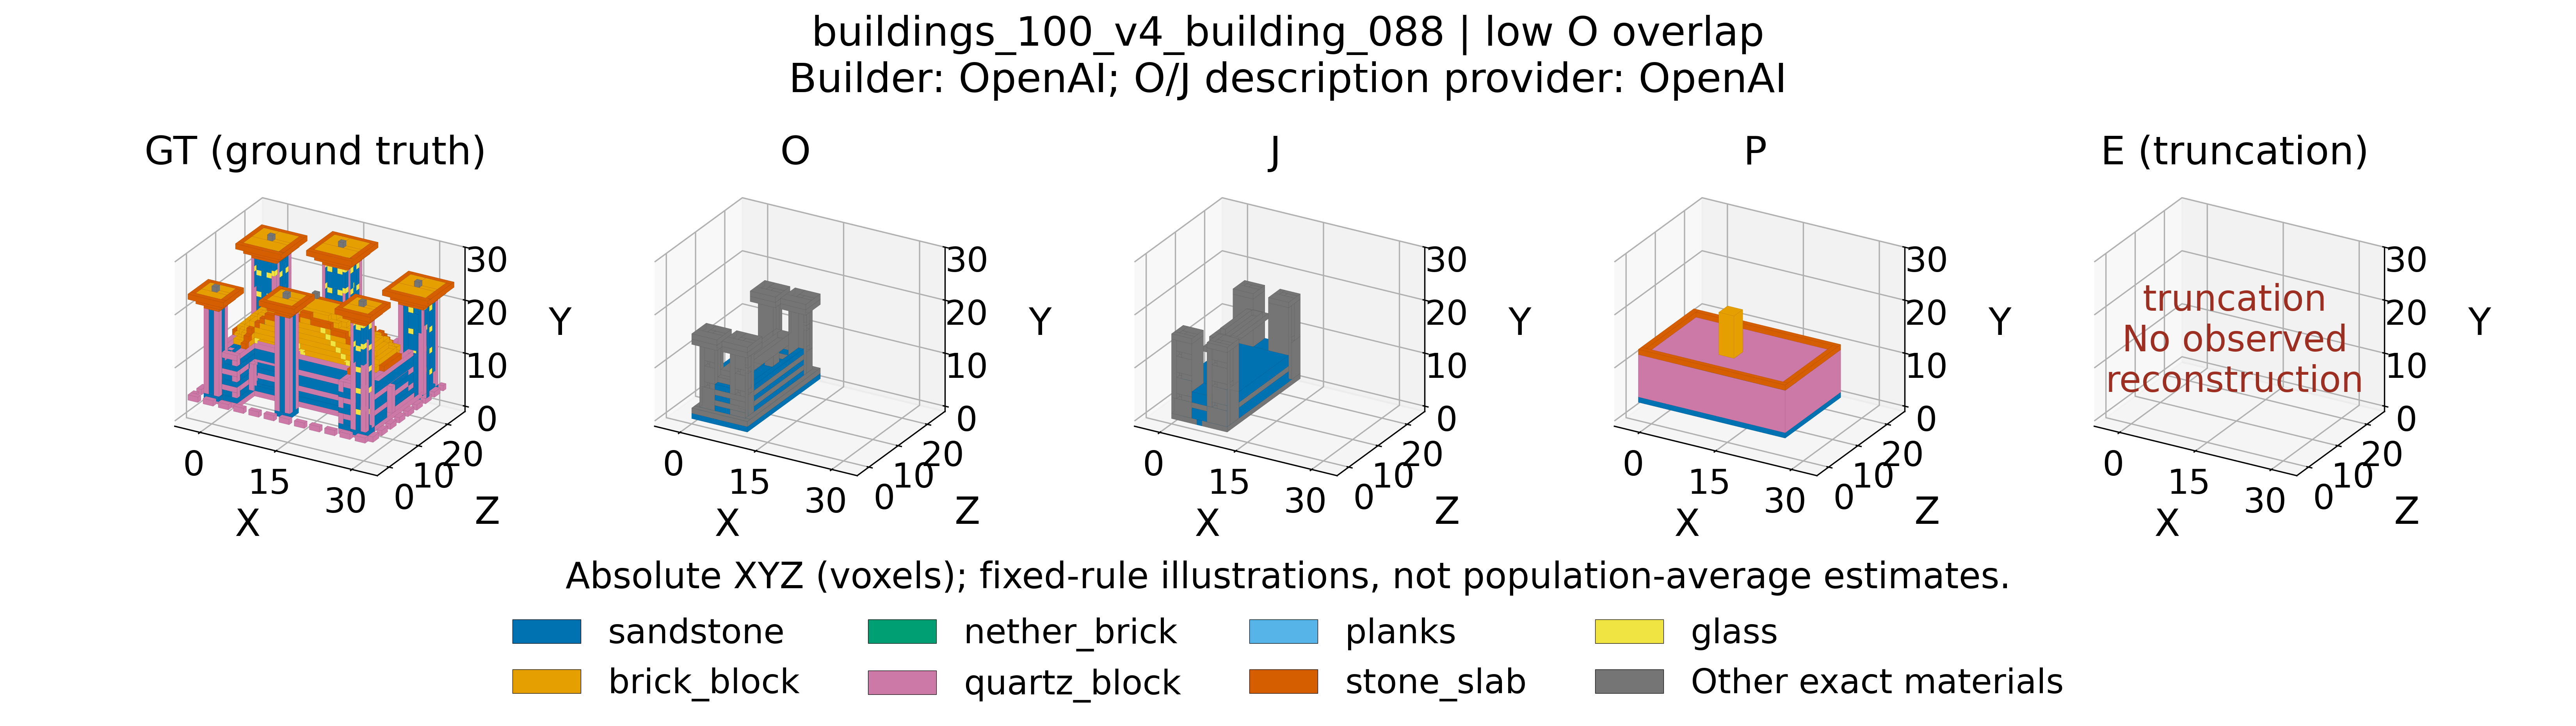
\includegraphics[width=\textwidth]{example_02.png}\\[2pt]
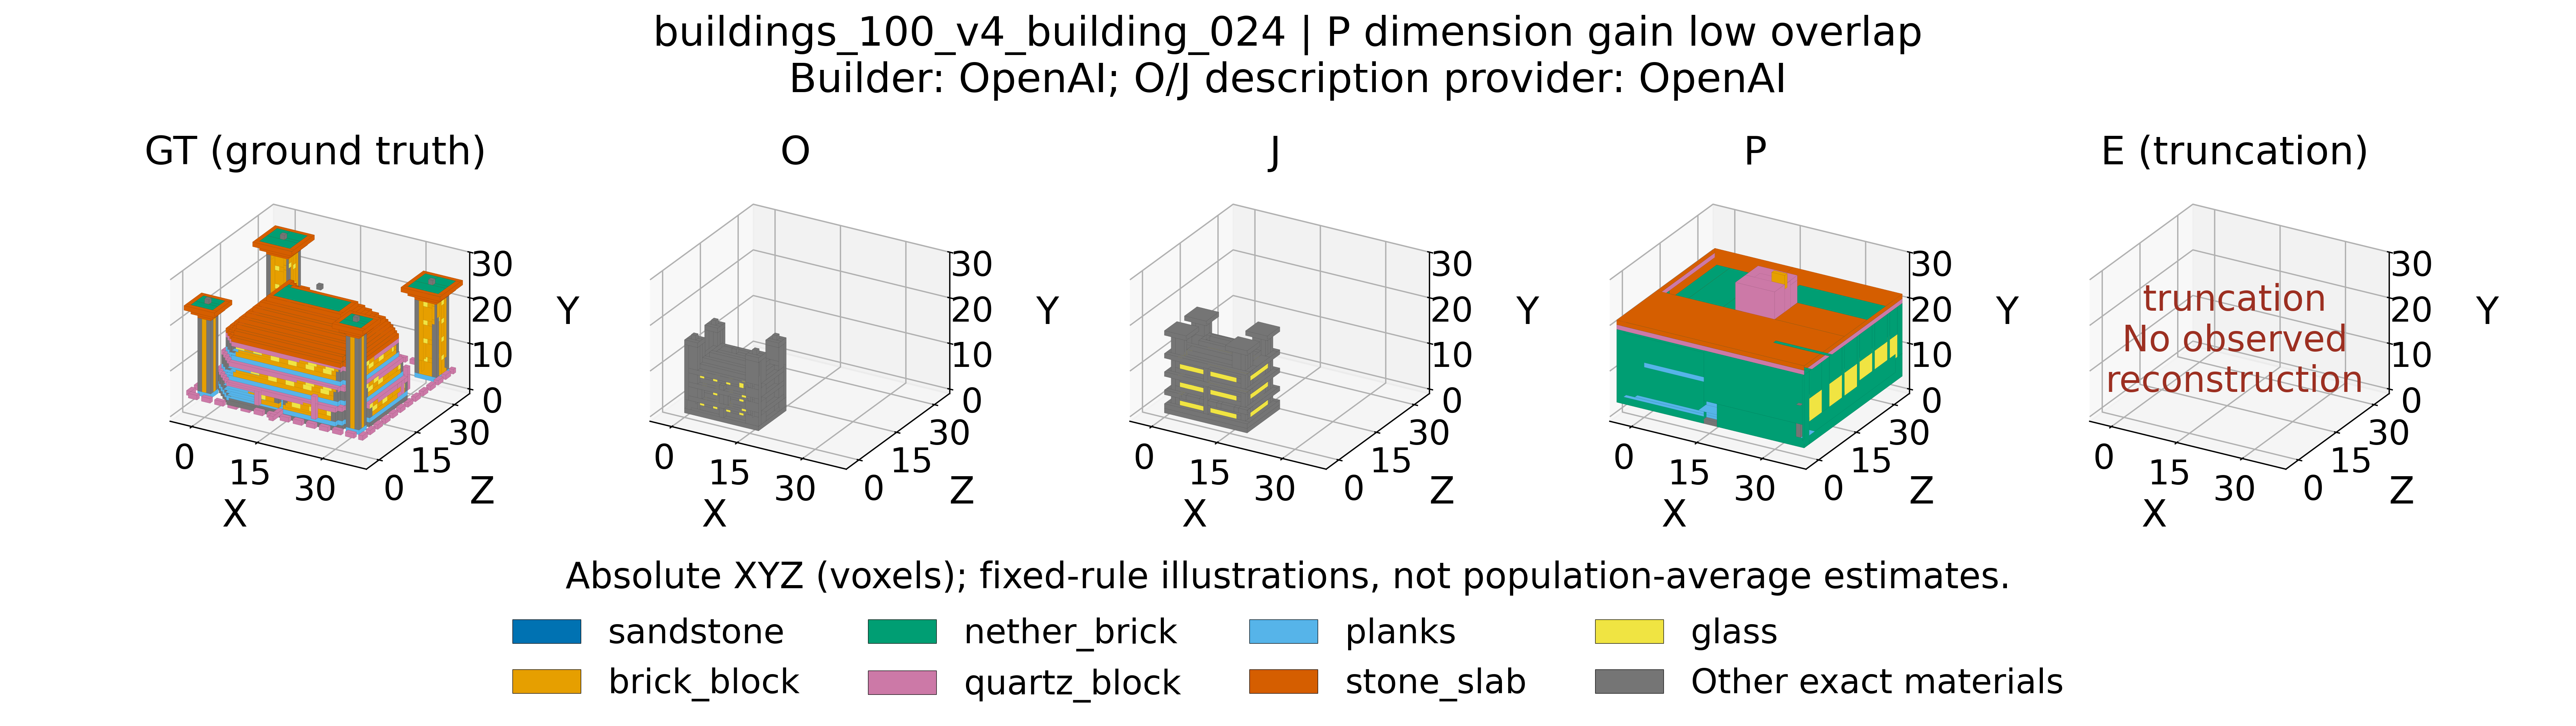
\includegraphics[width=\textwidth]{example_03.png}
\caption{Three distinct buildings selected by the fixed near-median O, low-O-overlap,
and P-dimension-gain with P IoU at most 0.20 rules, respectively.
All panels use unmodified absolute world coordinates, a common orthographic camera,
and identical axes and voxel scale within each row. The stored strict-aligned metrics
were used for selection only. O is the saved JSON-form visual description record;
J preserves that JSON tree; P/E supply partial/full GT information.
Failed E outputs remain explicitly marked, with no invented geometry.
Colors group the seven most frequent exact GT materials and other materials for display
only; exact identities and metrics remain in the source table.
These illustrative examples do not estimate population-average performance.
Source hashes, literal description excerpts, metrics and per-panel provenance appear in
the accompanying example table and manifest.}
\label{fig:goal008-reconstruction-examples}
\end{figure*}
